% -*- root: ../../main.tex -*-
%!TEX root = ../../main.tex
% vim:textwidth=80 fo=cqt

In  order  to  establish  a  context  for the  author's  work  to  be  discussed
in  \cref{ch:newelectrolytemodel},  it  is  imperative  to  provide  a  holistic
presentation of the basic \gls{spm} modelling art. The conventional \gls{spm} is
the  simplest  of  all  time  domain  \glspl{pbm}.  The  rest  of  this  section
provides  this author's  digested summary  of its  modelling rubrics  based upon
the  keen  insights  gained  from  perusing  the  vanguard  literature  in  this
topic~\cite{Santhanagopalan2006,Santhanagopalan2006a,DiDomenico2010} as  well as
their relevant derivative works.

\subsection{Geometry}\label{subsec:basicspmgeometry}

A  description  of   the  working  principle  of  the  cell   was  presented  in
\cref{subsec:liionchemistry} and  is not  repeated here.  The \gls{spm}  aims to
capture the electrochemical phenomena along the thickness~$l_j$,~\jinnegpos{} of
each  porous electrode  by a  representative  spherical particle.  Thus the  two
distinct  solid  phase porous  regions  of  the  cell \ie~the  negative  and
positive electrode regions, are idealised as two spheres of radii~$R_\text{neg}$
and~$R_\text{pos}$ respectively.


\Cref{fig:sandwichtospm}   shows   the   geometrical  origins   of   the   basic
\gls{spm}.  In  this   arrangement,  the  spatial  dimension   along  the  axial
thickness  of   each  electrode   degenerates  to  a   single  point   which  is
represented  by  a sphere.  Hence,  the  concentration  of Lithium  within  each
electrode~$c_{\text{s}_j}$,~\jinnegpos{}  is  only  a  function  of  the  radial
position~$r_j$,~\jinnegpos{}  and  the  time~$t$.   The  surface  area  of  each
representative sphere is scaled appropriately,  such that they are equivalent to
the  active area  of the  corresponding  porous electrodes.  Thus the  \gls{spm}
accounts  for  the  reduced  volume-fraction  arising  due  to  the  microporous
structure  of  the   solid  phase  and  hence,  the  storage   capacity  of  the
representative  particles  match  that  of  the  corresponding  electrodes.  The
overarching  assumption  of  the  \gls{spm} modelling  philosophy  is  that  the
electrochemical performance of these representative electrodes are sufficient to
model the behaviour of the cell at its terminals. The \gls{spm} thus employs the
coarsest possible spatial  discretisation of the cell's thickness  with the goal
of minimising computational burden.

\begin{figure}[!htbp]
    \centering
    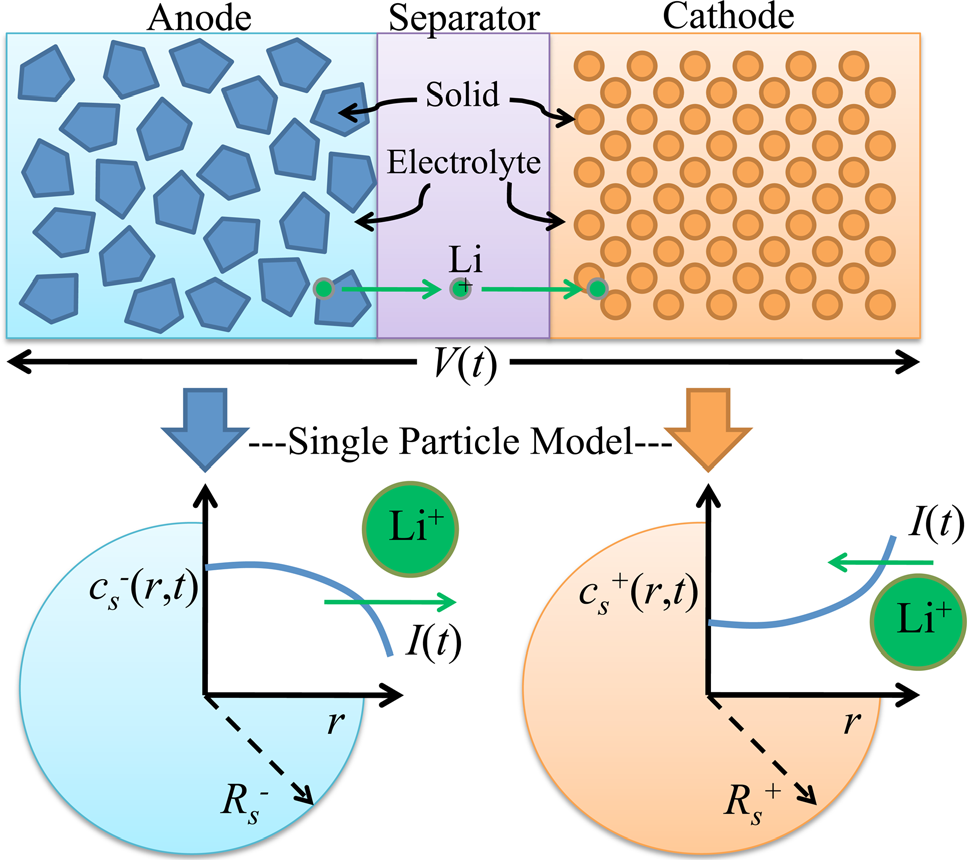
\includegraphics{spm_geometry}
    \caption[Schematic illustration depicting geometrical origins of the
    \glsfmtshort{spm}]
    {%
        Schematic illustration depicting the geometrical origins of the basic
        \gls{spm}. The model is obtained through a degenerate spatial
        discretisation of one electrochemical layer of a  pouch cell.  The
        active material of each porous electrode is represented by one
        representative spherical particle, thus entirely eliminating the spatial
        dimension along the axial direction. Illustration reproduced
        from Moura~\etal~\cite{Moura2012}.
    }%
    \label{fig:sandwichtospm}
\end{figure}

\subsection{Scope and Assumptions}\label{subsec:basicspmassumptions}

Having described the  geometrical representation of the model,  it is imperative
to establish its  aims and scope. This section discusses  the subset of physical
phenomena  that can  be  captured  by the  basic  \gls{spm}  and enumerates  the
inherent assumptions in model derivation.  The validity of these assumptions and
their effects  on model accuracy shall  be examined in the  results presented in
\cref{subsec:simresultsbasicspm}. As  a broad  outline of  its scope,  the model
attributes  the  cell polarisation  to  two  dominant physics,  \viz~reaction
kinetics and solid phase transport phenomena \ie~diffusion dynamics.


The  \gls{spm}  assumes that  charge  transfer  happens throughout  the  surface
of  each  representative  spherical  particle where  intercalation  occurs.  The
electronic  conductivity of  the solid  phase is  assumed to  be high  enough to
ignore the  spatial distribution  of charge \ie~the local  volumetric current
density is assumed  to be uniform along the thickness  of each porous electrode.
This assumption is  motivated by the early calculations performed  by Newman and
Tobias~\cite{Newman1962} in their stand-alone  analysis of current distributions
in porous electrodes, wherein a volume-averaged molar flux was deemed sufficient
throughout  the  thickness  of  the  electrode.  This  uniform  current  density
assumption implies  that all of the  particles in the electrode  active material
are  in parallel.  Solid  phase  diffusion dynamics  within  each electrode  are
therefore solved by assuming this averaged electrochemical reaction rate. In the
simulation study  by Smith and~Wang~\cite{Smith2006},  it is reported  that soon
after  the beginning  of discharge,  solid  phase concentration  and ionic  flux
become nearly  independent of  spatial position, and  that Lithium  diffusion in
solid particles may be driven by an averaged molar flux at the surface.


Based  on the  discussion thus  far, it  is clear  that the  \gls{spm} does  not
attempt to  model all  physical processes  within the  cell. In  particular, the
model assumes  instantaneous charge  transport from one  electrode to  the other
through  the  solution  phase.  This  implies  that  electrolytic  diffusion  is
sufficiently  fast  (relative to  diffusion  in  the  solid phase).  Thus,  mass
transport  phenomena  in  the  electrolyte  have been  neglected  in  the  basic
\gls{spm}.


During   the  operation   of  the   cell,   the  \gls{spm}   assumes  that   the
electrolyte  concentration~$c_\text{e}$  remains  constant  at  its  equilibrium
initial value~$c_{\text{e},0}$  throughout the cell thickness.  Neglecting local
concentration gradients in  the solution phase, together with  ignoring its mass
transport phenomena, implies  that the current in the electrolyte  does not vary
over  space  and  time.  Hence,  in  the  conventional  \gls{spm}  there  is  no
contribution of the solution phase  to internal overpotentials \ie~electrolyte
dynamics have  no influence on the  cell's terminal voltage. The  \gls{spm} also
ignores any  variations in material  porosities in each  electrode. Furthermore,
all solid phase diffusivities and kinetic parameters are held constant. Finally,
all thermal effects are assumed to  be negligible and no degradation effects are
attempted to be modelled in the basic \gls{spm} formulation.

These  simplifying  assumptions  are  made  so as  to  facilitate  the  ease  of
implementing a  \gls{pbm}, without incurring  the heavy computational  cost that
typically accompanies it. The impact of these assumptions on the accuracy of the
model shall  be examined in \cref{subsec:simresultsbasicspm}  and later sections
presents prior research that strives to  straddle the fine balance between model
sophistication and computational complexity.

\subsection{Governing  Equations}\label{subsec:basicspmgoverningeqns}
% {Governing  Equations\protect\footnote{In  this
% section,   only  those   simplifications  to   mathematical  notations   arising
% due  to  assumptions  discussed  in \cref{subsec:basicspmassumptions}  shall  be
% introduced   in-line.   For  a   comprehensive   reference   to  the   notations
% used,   please  refer   to   nomenclature   list  in   the~\nameref{ch:glossary}
% chapter.  Notations  introduced  solely  for   this  section  are  also  covered
% here.}}


As discussed  in \cref{subsec:basicspmassumptions},  the \gls{spm}  captures the
cell's dynamics arising due to diffusion  and kinetics at the two representative
spherical electrodes. It also accounts for the contribution of their equilibrium
thermodynamics to the cell's \gls{ocp}.

\subsubsection*{Solid Phase Diffusion}

Conservation of \ch{Li^0} in the electrodes can be obtained by assuming that the
movement of neutral  atoms within the solid phase is  primarily due to diffusion
within particles.  This diffusion  phenomena is induced  due to  a concentration
gradient that  exists between the surface  and interior/core of the  solid phase
particles. Based on the geometrical assumptions of the \gls{spm} as discussed in
\cref{subsec:basicspmgeometry} \ie~owing to the lack of spatial discretisation
in  the  axial  direction~$x$,  the  concentrations  of  \ch{Li^0}  in  the  two
electrodes~$c_\sj(x,r,t)$, reduce  to a  function of the  radial co-ordinate~$r$
and time~$t$, and is denoted by~$c_\sj(r,t)$,~\jinnegpos{}. To keep the notation
tractable, this  explicit spatio-temporal radial dependence  is omitted, further
simplifying the representation  to~$c_\sj$. We start with the  derivation of the
solid-phase diffusion equation \cref{eq:dfnsoliddiff} in \cref{tbl:dfneqns}, and
then proceed  to the simplifications  of its boundary conditions  facilitated by
the \gls{spm} assumptions.

Diffusion  in the  solid phase  can be  modelled by  applying classical  Fickian
dynamics~\cite{Fick1995} given by
\begin{equation}\label{eq:cartesiandiffusion}
    \diffp{c_\sj}{t} = ∇\! ⋅ \left(D_\sj\, ∇ c_\sj \right)\qquad \jinnegpos{}%\footnotemark{}
\end{equation}
% \footnotetext{For  the  sake of  brevity,  in  rest  of  the equations  in  this
% section,  the  explicit  definition  for   each  subsequent  occurrence  of  the
% subscripted variable $j$ shall be omitted. It is implied that \jinnegpos{} since
% these  equations describe  solid phase  diffusion in  the negative  and positive
% electrodes.}
The  divergence of  a vector  field~$\mathbf{F}(r,θ,ϕ)$ can  be expressed  in
spherical co-ordinates as
\begin{equation}\label{eq:fullsphericaldiv}
    ∇ ⋅ \mathbf{F} = \frac{1}{r^2}\diffp{\left(r^2 F_r\right)}{r} +
    \frac{1}{r \sin θ}\diffp{\left(\sin θ\:  F_θ\right)}{θ}
    + \frac{1}{r \sin θ}\diffp{F_ϕ}{ϕ}
\end{equation}
where  $r$~denotes the  radius,  $θ$~the polar  angle,  and $ϕ$~the  azimuthal
angle. $F_r, F_θ$ and $F_ϕ$~denote  the corresponding components of the vector
field~$\mathbf{F}$.

The  co-ordinate  origin  at  each  electrode is  aligned  with  the  centre  of
its  representative  spherical  particle.  Due  to symmetry  in  the  polar  and
azimuthal axes, the  divergence becomes a function of only  the radial position.
\Cref{eq:fullsphericaldiv} therefore reduces to
\begin{equation}\label{eq:reducedsphericaldiv}
    ∇ ⋅ \mathbf{F} = \frac{1}{r^2}\diffp{\left(r^2 F_r\right)}{r}
\end{equation}
Applying     the     \gls{rhs}     of     the     divergence     operator     of
\cref{eq:reducedsphericaldiv} in \cref{eq:cartesiandiffusion} yields
\begin{equation}\label{eq:csdiffusioneqn}
    \diffp{c_\sj}{t} = \frac{1}{r^2}\diffp*{\left(r^2 D_\sj\, ∇ c_\sj \right)}{r}
\end{equation}
As   per  the   assumption  of   uniform   diffusivity  in   the  solid   phase,
\cref{eq:csdiffusioneqn} becomes
\begin{align}
    \diffp{c_\sj}{t} &= \frac{D_\sj}{r^2}\diffp*{\left(r^2 ∇ c_\sj \right)}{r}\label{eq:csdiffusionconstdiffusivity}
    \intertext{Applying the gradient operator of \cref{eq:csdiffusionconstdiffusivity} along
    the radial direction~$r$,}
    \diffp{c_\sj}{t} &= \frac{D_\sj}{r^2}\diffp*{\left(r^2 \diffp{c_\sj}{r} \right)}{r}\label{eq:csdiffusionfinal}
\end{align}
\Cref{eq:csdiffusionfinal} represents  a mass-balance equation  describing solid
phase diffusion  in each electrode  and is  identical to the  governing equation
\cref{eq:dfnsoliddiff} from \cref{tbl:dfneqns}. The  potential at each electrode
depends  on   the  solid  phase  surface   concentration~$c_\sjsurf$  \ie~the
\ch{Li^0} concentration~$c_\sj(r,t)$  evaluated at~$r=R_\pj$,~\jinnegpos{} where
$R_\pj$~represents  the  equivalent  radius  of  each  representative  spherical
particle.

Due to spherical symmetry,  flux at the centre of the  particle is considered to
be zero.
\begin{equation}\label{eq:csfluxcentre}
    \diffp{c_\sj}{r}{\mathrlap{r=0}} = 0
\end{equation}

Diffusion in the solid phase is driven by concentration gradients induced due to
intercalation flux  density at the  particle surface  \ie~the surface  of each
particle experiences a pore-wall flux density driven by reaction kinetics. Based
on  the  \gls{spm}  geometry discussed  in  \cref{subsec:basicspmgeometry},  the
spatial dependence of this molar  flux density~$j_\nj(x,t)$ is eliminated and it
can  therefore  be  represented  as~$j_\nj(t)$,~\jinnegpos{}. For  the  sake  of
brevity,  its  explicit temporal  dependence  is  also  omitted resulting  in  a
simplified notation~$j_\nj$. Hence, at the particle surface
\begin{equation}\label{eq:csfluxsurface}
    D_\sj\diffp{c_\sj}{r}{\mathrlap{r=R_\pj}} = -j_\nj
\end{equation}
The sign convention chosen here is such that pore-wall flux leaving the particle
surface is considered to be positive.

Charge   conservation   in   solid   phase    is   applied   to   evaluate   the
\gls{rhs}  in \cref{eq:csfluxsurface},   a  detailed  derivation  of   which  is
presented  in  Domenico~\etal~\cite{DiDomenico2010}.  In  summary,  by  assuming
a  uniform   charge  density   throughout  the   thickness  of   each  electrode
(see \cref{subsec:basicspmassumptions}), we get
\begin{align}
    j_\nj(t)                       &= ± \frac{I(t)}{A \, l_j a_\sj F}\label{eq:uniformcurrdensity}   \qquad \jinnegposordered
    \intertext{Substituting \cref{eq:uniformcurrdensity} in \cref{eq:csfluxsurface}}
    D_\sj\diffp{c_\sj}{r}{\mathrlap{r=R_\pj}} &= ∓ \frac{I}{A \, l_j a_\sj F}\label{eq:csfluxsurfacefinal} \qquad \jinnegposordered
\end{align}
wherein  the  load current~${I(t)  >  0}$  for discharge,  whose  explicit
time-dependence  has  been  omitted in  \cref{eq:csfluxsurfacefinal}  for  being
consistent notation with the \gls{lhs}. The positive and negative signs apply to
the negative  and positive  electrode respectively as  indicated by  the ordered
pair \jinnegposordered. It  should be noted that the term  involving the Faraday
constant in the \gls{rhs}  of \cref{eq:uniformcurrdensity} is~$nF$, where $n$~is
the number  of electrons  transferred during the  reaction. However,  since this
thesis only  discusses lithium-ion  chemistries where~$n=1$, this  is implicitly
conveyed and shall be omitted for all potential occurrences.

The \gls{soc} of the cell can be obtained from the bulk concentration of lithium
in  either the  negative  or  positive electrode.  By  convention, the  negative
electrode is used.
\begin{equation}\label{eq:socinitialdefn}
    z(t) = \frac{3}{c_\snegmax}∫_0^{R_\pneg}r^2 c_\sneg (r,t)\, dr
\end{equation}
Given an  initial cell  \gls{soc}~${z(0) = z_0}$  at rest,  the equilibrium
concentration of \ch{Li^0} in the two individual electrodes can be computed as
\begin{equation}\label{eq:csfluxinitialcondition}
    c_\sj(r,0) = c_\sjmax \, \bigg[z_0 \left(θ_\maxj - θ_\minj \right) + θ_\minj \bigg]
\end{equation}

\Cref{eq:csdiffusionfinal},          its         corresponding          boundary
conditions~\eqref{eq:csfluxcentre} and~\eqref{eq:csfluxsurfacefinal}  along with
initial   condition~\eqref{eq:csfluxinitialcondition},   provide  the   complete
description of  time-domain evolution of  lithium in the  conventional \gls{spm}
for  a  given  applied  current  profile~$I(t)$.  Considerations  for  efficient
numerical simulation of this system is presented next.

%  in \cref{subsec:basicspmgeometry}.


\subsubsection*{Further Reduction in Dimensionality}\label{subsec:basicspmfurtherdimensionalityreduction}

A naive approach to numerically solving the solid phase diffusion equation is to
discretise each of the two representative particles in the radial direction~$r$.
Given the elaborate  simplifications made to remove spatial  resolution from the
axial  direction, the  efficacy of  using  a radial  discretisation is  rendered
questionable, particularly within the scope of  embedding the model in an online
simulation and  state-estimation environment. Since diffusion  in each spherical
particle is modelled by the well-known Fickian dynamics~\cite{Fick1995}, several
attempts have  been made to  obtain an  approximate analytical solution  for the
solid phase concentration in both electrodes.
% In  the  context  of  \gls{spm}  modelling, the  earliest  such  work \ie~a
% comparison of  the discretised version  with an approximate  analytical solution
% was performed by Santhanagopalan~\etal~\cite{Santhanagopalan2006}.
In a  dimensionless analysis study,  Zhang and White~\cite{Zhang2007}  provide a
comparative  evaluation of  the various  approximation methods  for solid  phase
diffusion, a summary of which is presented in \cref{tbl:solidphaseapprox}.

% -*- root: ../main.tex -*-
%!TEX root = ../main.tex

\begin{table}[!htbp]
    \caption[Solid phase diffusion approximation methods]{Summary of approximation methods for solid phase diffusion}
    \label{tbl:solidphaseapprox}
    \centering
    \begin{tabular}{@{}ll@{}}\toprule
        Method                     & Introduced by                                             \\ \midrule
        Duhamel's superposition    & Doyle, Fuller \&  Newman~\cite{Doyle1993,Fuller1994}      \\
        Diffusion length           & Wang~\etal~\cite{Wang1998}                                \\
        Corrected Diffusion length & Wang and Srinivasan~\cite{Wang2002}                 \\
        Polynomial approximation   & Subramanian~\etal~\cite{Subramanian2001a,Subramanian2005} \\
        Pseudo steady-state        & Liu~\cite{Liu2006}                                        \\
        \bottomrule
    \end{tabular}
\end{table}


In  the   aforementioned  study,   the  computational  burden,   \viz~storage
requirements and  CPU times of  Duhamel's superposition  method was found  to be
excessively  high to  warrant further  interest  in it.  The original  diffusion
length method proposed  by Wang~\etal{} is valid only after  the diffusion layer
builds  up  to its  steady  state,  and hence  leads  to  significant errors  in
transient  conditions.  Although Wang  and  Srinivasan  introduced an  empirical
correction factor to  the diffusion length to extend its  validity to short-time
scale operations, this  affected the convergence of the method  for steady state
conditions.  The pseudo  steady state  solution proposed  by Liu  uses a  finite
integral  transform  technique  to  eliminate the  radial  dependence  of  solid
phase concentration.  However, this method uses  computations involving infinite
summations,  exponential  and trigonometric  quantities,  which  in this  thesis
author's view, makes it less attractive for online implementations.

The         literature         on          polynomial         methods         by
Subramanian~\etal{}~\cite{Subramanian2005} provide  detailed derivations  of the
\engordnumber{2}~and   \engordnumber{4}~order  polynomial   approximations.  The
\engordnumber{2}~order solution was found to have poor performance for transient
behaviour, similar  to that  of the original  diffusion length  method. However,
higher order polynomial  approximations were found to  provide acceptable levels
of  performance  for  both  transient  and steady  state  conditions  and  shall
therefore be examined further.

The  polynomial   approximation  method  describes  the   dynamic  evolution  of
the  volume  averaged concentration
\begin{equation}
    c_\sjavg(t)  = \frac{1}{Ω}  ∫\limits_Ω c_\sj(r,t)\,  dΩ
\end{equation}
as  a function  of the  applied load  current~$I(t)$. Here,  $Ω$~represents the
volume  of  the spherical  particle.  For  notational brevity,  $c_\sjavg(t)$~is
shortened to $\mean{c}_\sj$~whilst also dropping its explicit time dependence.

The \engordnumber{4}~order polynomial approximation assumes that the solid phase
concentration~$c_\sj(r,t)$ is a quartic function of the radial co-ordinate~$r$.
\begin{equation}\label{eq:fourthorderpoly}
    c_\sj(r,t) = a(t) + b(t)\left(\frac{r}{R_\pj}\right)^2 + d(t) \left(\frac{r}{R_\pj}\right)^4
\end{equation}

The    detailed   derivation    of   the    coefficients~${a(t),    b(t)
\text{ and } c(t)}$     is     provided    in     Subramanian~\etal{}~\cite{Subramanian2005}.
\Cref{eq:csmeanevolution,eq:qmeanevolution,eq:csurffromcsavg}    summarise   the
governing equations  obtained by applying the  \engordnumber{4}~order polynomial
approximation of \cref{eq:fourthorderpoly}  to the system of  equations given by
\cref{eq:csdiffusionfinal,eq:csfluxcentre,eq:csfluxsurfacefinal}.
\begingroup
\allowdisplaybreaks
\begin{align}
    \diff*{\mean{c}_\sj}{t} + 3\frac{j_\nj}{R_\pj}                                                &=0 \label{eq:csmeanevolution} \\
    \diff*{\mean{q}_j}{t} + 30\frac{D_\sj}{R_\pj^2}\mean{q}_j + \frac{45}{2}\frac{j_\nj}{R_\pj^2} &=0 \label{eq:qmeanevolution}\\
    35\frac{D_\sj}{R_\pj}\left(c_\sjsurf - \mean{c}_\sj\right) - 8D_\sj \mean{q}_j                &= -j_\nj \label{eq:csurffromcsavg}
\end{align}%
\endgroup
where $\mean{q}_j(t)$~represents  the volume  averaged concentration  flux, that
defines  the  average  change  of  concentration  with  respect  to  the  radial
position~$r$.

As   per  \cref{eq:uniformcurrdensity},   the   interfacial   flux  density   is
proportional to  the applied current. Hence  \cref{eq:csmeanevolution} implies a
simple linear relationship between the applied current and the rate of evolution
of average \ch{Li^0} concentration within  each spherical particle. This further
implies  that the  \gls{soc} of  the cell  has a  linear rate-dependence  on the
externally  applied  current. Furthermore,  due  to  the elimination  of  radial
discretisation, the computation of \gls{soc}, given by \cref{eq:socinitialdefn},
reduces to the task of first computing the ratio of bulk (average) concentration
to  surface concentration  and  then adjusting  it to  account  for the  useable
stoichiometry limits for the relevant electrode. Thus, the cell's \gls{soc}
% as predicted by the \gls{spm}
can be computed as
\begin{equation}\label{eq:soccomputation}
    z = \frac{\tfrac{\mean{c}_\sneg}{c_\snegmax} - θ_\minneg}{θ_\maxneg - θ_\minneg}
\end{equation}
where $\mean{c}_\sneg$~is obtained by  solving \cref{eq:csmeanevolution} for the
negative electrode.

In   the  views   of   this  author,   this  \engordnumber{4}~order   polynomial
approximation   proposed  by   Subramanian~\etal~\cite{Subramanian2005}  strikes
an  acceptable  balance  between   the  three  modelling  pivots ---
\begin{enumerate*}[label=\roman*)]
    \item computational complexity,
    \item mathematical  tractability, and
    \item numerical accuracy
\end{enumerate*}
and has therefore  been adopted for all \gls{spm} simulations  presented in this
work.

At   the   end   of    this   dimension-reduction   step,   spatial   dependence
is   completely  eliminated,   yielding   a  zero-order   (in  space)   physical
model    whose    dynamics   are    described    by    the   \gls{dae}    system
of \cref{eq:csmeanevolution,eq:qmeanevolution,eq:csurffromcsavg}.

% Thermodynamics, kinetics and state-space formulation  of the model are presented
% next in \cref{subsec:basicspmthermodynamics}.

\subsubsection*{Equilibrium Thermodynamics}\label{subsec:basicspmthermodynamics}

The equilibrium potential of a porous electrode is a thermodynamic property that
depends on the extent of lithiation in the outermost interstitial sites near the
\gls{sei} layer. This surface stoichiometry~$θ_j$  for an electrode is obtained
by  computing the  surface  concentration  (using \cref{eq:csurffromcsavg})  and
dividing by the maximum lithiation capacity of that electrode.
\begin{equation}
    θ_j = \frac{c_\sjsurf}{c_\sjmax}
\end{equation}

Although based upon the theoretical foundation  laid out by the Nernst equation,
owing  to a  multitude of  complex phase  transitions, the  potential of  porous
electrodes  (with respect  to metallic  lithium) is  usually given  as empirical
functions of its surface stoichiometry~\cite{Reddy2011,Rahn2013}.
\begin{equation}\label{eq:ocpstoichiometry}
    U_j(t) = \mathcal{U}_j\left(θ_j(t)\right)
\end{equation}
where  the  empirical  relationships~$\mathcal{U}_j$ are  typically  high  order
polynomials  or rational  functions  that  are fitted  to  relaxation data  from
\gls{gitt} experiments on half-cells~\cite{Birkl2015a,Ecker2015}.

In the \gls{spm},  the cell's \gls{ocp} is obtained by  subtracting the negative
electrode  equilibrium  potential~$U_\text{neg}$  from  its  positive  electrode
counterpart~$U_\text{pos}$.
\begin{equation}\label{eq:ocpdefinition}
    U_\text{ocp} = U_\text{pos} - U_\text{neg}
\end{equation}
Even though the  concept of \gls{ocp} is defined only  in equilibrium conditions
when no  current flows,  the individual electrode  potentials themselves  form a
significant component of the cell's terminal voltage~$V(t)$.

\subsubsection*{Reaction Kinetics}

In the \gls{spm}, the reaction kinetics in each spherical electrode is modelled
using the Butler-Volmer expression (see \cref{eq:butlervolmer}).
\begin{align}
    j_\nj   &= j_{0_j} \left[ \exp\left( \frac{\left(1-α\right) F η_j}{R T}\right) -  \exp\left( \frac{-α F η_j}{R T}\right)\right] \label{eq:bvwithalpha} \\
    \shortintertext{where}
    j_{0_j} &= k_\jr c_\text{e}^{1-α} c_\sjsurf^{α} \left(c_\sjmax - c_\sjsurf\right)^{1-α}
\end{align}

The equilibrium  rate of forward  and backward  reactions at both  electrodes is
assumed  to  be  equal.  With charge  transfer  coefficient~${α  =  0.5}$,
\cref{eq:bvwithalpha} simplifies to
\begin{equation}\label{eq:BVwithalphahalf}
    j_\nj = 2 k_\jr \sqrt{c_\text{e} c_\sjsurf \left(c_\sjmax - c_\sjsurf\right)} \sinh\left(\frac{F η_j}{2 R T}\right)
\end{equation}

The  expression   for  overpotential~$η_j$   can  be   obtained  rearranging by
\cref{eq:BVwithalphahalf}     whilst     substituting    for     $j_\nj$~from by
\cref{eq:uniformcurrdensity} and is given                                     by
\begin{equation}\label{eq:overpotential_j}
    η_j(t) =  \frac{2 R T}{F }\sinh^{-1} \left( \frac{± I(t)}{2 A \, l_j a_\sj F k_\jr \sqrt{c_\text{e} c_\sjsurf \left(c_\sjmax - c_\sjsurf\right)}}\right)
\end{equation}

\subsubsection*{Cell Terminal Voltage}\label{subsec:basicspmcellterminalvoltage}

The terminal voltage  of the cell under applied load  is obtained by subtracting
the potential of the negative electrode from its positive counterpart.

Starting from the definition of the overpotential of each electrode
\begin{align}
    η_\text{pos} &= ϕ_\spos - \cancelto{0}{ϕ_\epos} - U_\text{pos} \label{eq:posoverpotential} \\
    η_\text{neg} &= ϕ_\sneg - \cancelto{0}{ϕ_\eneg} - U_\text{neg} \label{eq:negoverpotential}
\end{align}
Within  each electrode  domain,  the contribution  of  electrolyte potential  is
neglected  (see \cref{subsec:basicspmgeometry,subsec:basicspmassumptions}  for a
brief discussion on the exclusion of electrolyte dynamics).

Subtracting \cref{eq:negoverpotential}   from \cref{eq:posoverpotential},
% whilst substituting for $U_j$ from \cref{eq:ocpstoichiometry}
\begin{align}
    η_\text{pos} - η_\text{neg} &= \underbrace{ϕ_\spos - ϕ_\sneg}_{V_\text{cell}} - U_\text{pos} + U_\text{neg}\label{eq:overpotentialdifference}\\
\shortintertext{whose rearrangement yields}
    V_\text{cell}               &= η_\text{pos} - η_\text{neg} + U_\text{pos} - U_\text{neg}\label{eq:cellterminalvoltagebasic}
\end{align}
% \mathcal{U}_\text{pos}\left(θ_\text{pos}\right) - \mathcal{U}_\text{neg}\left(θ_\text{neg}\right)
In the  basic \gls{spm},  \cref{eq:cellterminalvoltagebasic} is used  to compute
the cell's terminal voltage under  load. Although their explicit time-dependence
notation  is omitted  in  the notation  here,  it is  worth  reminding that  all
quantities in \cref{eq:cellterminalvoltagebasic} are indeed continuous functions
of time.

\subsubsection*{State Space Representation}\label{subsec:basicspmstatespace}

For control  oriented applications, it is  imperative to have a  classical state
space representation  that collates  all intermediate equations  and definitions
presented  thus  far into  a  single  system  of  equations that  describes  the
evolution of solid concentration and terminal  voltage over time, expressed as a
response to the  external current input~$I(t)$. However,  the non-linearities in
the equation for terminal voltage \ie~\cref{eq:cellterminalvoltagebasic} imply
that it is  not possible to represent  the \gls{spm} in the form  of a classical
\gls{lti}  system  of \cref{eq:LTIstatespace}.  Instead,  the  \gls{spm} can  be
summarised  by a  system  of linear  state equations  together  with the  single
non-linear output equation.

Rearranging  \cref{eq:qmeanevolution,eq:csurffromcsavg}, the  state equation  is
obtained as
\begin{equation}\label{eq:fourstatesmatrixvec}
    \setstackgap{L}{1.5\baselineskip}
    \fixTABwidth{T}
    \diff*{\parenMatrixstack{
            \vphantom{\frac{45}{2} \frac{1}{R_\ppos^2 A \, l_\text{pos} a_\spos F}}
            \mean{q}_\text{pos} \\
            \vphantom{\frac{45}{2} \frac{1}{R_\ppos^2 A \, l_\text{pos} a_\spos F}}
            % \vphantom{\frac{D_\sneg}{R_\pneg^2}}
            \mean{q}_\text{neg} \\
            \vphantom{\frac{45}{2} \frac{1}{R_\ppos^2 A \, l_\text{pos} a_\spos F}}
            % \vphantom{\frac{D_\spos}{R_\ppos^2}}
            \mean{c}_\spos \\
            \vphantom{\frac{45}{2} \frac{1}{R_\ppos^2 A \, l_\text{pos} a_\spos F}}
            % \vphantom{\frac{D_\sneg}{R_\pneg^2}}
            \mean{c}_\sneg
        }
    }{t}
    = \underbrace{\parenMatrixstack{
            -30\frac{D_\spos}{R_\ppos^2} & 0                            & 0 & 0 \\
            0                            & -30\frac{D_\sneg}{R_\pneg^2} & 0 & 0 \\
            \vphantom{\frac{45}{2} \frac{1}{R_\ppos^2 A \, l_\text{pos} a_\spos F}}
            0                            & 0                            & 0 & 0 \\
            \vphantom{\frac{45}{2} \frac{1}{R_\ppos^2 A \, l_\text{pos} a_\spos F}}
            0                            & 0                            & 0 & 0
    }}_{A}
    \parenMatrixstack{
        \vphantom{\frac{D_\spos}{R_\ppos^2}}
        \mean{q}_\text{pos} \\
        \vphantom{\frac{D_\sneg}{R_\pneg^2}}
        \mean{q}_\text{neg} \\
        \vphantom{\frac{D_\spos}{R_\ppos^2}}
        \mean{c}_\spos \\
        \vphantom{\frac{D_\sneg}{R_\pneg^2}}
        \mean{c}_\sneg
    }
    +
    \underbrace{\parenMatrixstack{
            \frac{45}{2} \frac{\hphantom{-}1}{R_\ppos^2 A \, l_\text{pos} a_\spos F} \\
            \frac{45}{2} \frac{-1}{R_\pneg^2 A \, l_\text{neg} a_\sneg F} \\
            \hphantom{\frac{45}{2}} \frac{\hphantom{-}3}{R_\ppos  A \, l_\text{pos} a_\spos F} \\
            \hphantom{\frac{45}{2}} \frac{-3}{R_\pneg  A \, l_\text{neg} a_\sneg F}
    }}_{B}
    I(t)
\end{equation}
which corresponds to the classical \gls{lti} form
\begin{equation}
    \dot{\mathbf{x}} = A\,\mathbf{x} + B\,\mathbf{u} \\
\end{equation}
where~${\mathbf{x}   =    \vect{\mean{q}_\text{pos},\mean{q}_\text{neg},
\mean{c}_\spos,  \mean{c}_\sneg},   \,  x  ∈  \mathbb{R}^{4   \times  1}}$  is
the  state  vector.  The  scalar system  input~$\mathbf{u}  ∈  \mathbb{R}$  is
the  applied  current~$I(t)$.  The  system matrix~${A  ∈  \mathbb{R}^{4  \times
4}}$  and  input  matrix~$B  ∈  \mathbb{R}^{4 \times  1}$  are  also  shown  in
\cref{eq:fourstatesmatrixvec}.

For state estimation and controller design purposes, it is important to keep the
number  of elements  in the  state vector  as small  as possible  by eliminating
redundant  variables.  For  instance,  Di~Dominico~\etal{}~\cite{DiDomenico2010}
noted that with  output voltage as the only measured  quantity, the observablity
of   the  four-state   model  of   \cref{eq:fourstatesmatrixvec}  is   adversely
affected.  To tackle  this issue,  a  state-reduction approach  was proposed  by
Di~Domenico~\etal~\cite{DiDomenico2010},  which  hinges  upon the  principle  of
material balance.

The total number of moles of lithium in the system is given by
\begin{equation}\label{eq:totallithiummoles}
    n_\text{Li} = \frac{ε_\spos \, l_\text{pos}\, A}{\frac{4}{3} π R_\ppos^3} ∫_0^{R_\ppos} 4 π r^2 c_\spos(r,t) \, dr
    +  \frac{ε_\sneg \, l_\text{neg}\, A}{\frac{4}{3} π R_\pneg^3} ∫_0^{R_\pneg} 4 π r^2 c_\sneg(r,t) \, dr
\end{equation}
Upon considering only the bulk concentration as per the dimensionality reduction
procedure    outlined   in \cref{subsec:basicspmfurtherdimensionalityreduction},
\cref{eq:totallithiummoles} reduces to
\begin{align}\label{eq:totallithiumsimplified}
    n_\text{Li}  &= \frac{ε_\spos \, l_\text{pos}\, A}{\frac{4}{3} π R_\ppos^3}\mean{c}_\spos ∫_0^{R_\ppos} 4 π r^2  \, dr
    + \frac{ε_\sneg \, l_\text{neg}\, A}{\frac{4}{3} π R_\pneg^3}\mean{c}_\sneg ∫_0^{R_\pneg} 4 π r^2  \, dr
                \\
                 &= ε_\spos \, l_\text{pos}\, A \, \mean{c}_\spos + ε_\sneg \, l_\text{neg}\, A \, \mean{c}_\sneg
\end{align}
Assuming    no    loss   of    cycleable    lithium    or   other    degradation
mechanisms,  the   total  number  of   moles  of   lithium  in  the   system  is
conserved   \ie~${\diff{n_\text{Li}}{t}   =  0}$.   Substituting   this   into
\cref{eq:totallithiumsimplified},
\begin{align}
    0                          &= \phantom{+} \diff*{ε_\spos \, l_\text{pos}\, A \, \mean{c}_\spos }{t} + \diff*{ε_\sneg \, l_\text{neg}\, A \, \mean{c}_\sneg }{t} \\
    \diff*{\mean{c}_\spos}{t}  &= -\diff*{\mean{c}_\sneg}{t} \label{eq:bulkconcrelationship}
\end{align}

As  per   \cref{eq:bulkconcrelationship},  the   time  evolution  of   the  bulk
concentration  of one  electrode can  be obtained  as a  function of  the other.
Furthermore, Di~Domenico~\etal{}~\cite{DiDomenico2010}  show that  the diffusion
dynamics of the  bulk concentrations can be algebraically  related through their
stoichiometric factors as
\begin{equation}\label{eq:csposbulkfromcsnegbulk}
    \mean{c}_\spos(t) = c_\sposmax \, \bigg[\frac{\mean{c}_\sneg(t)- θ_\minneg
    c_\snegmax}{\left(θ_\maxneg - θ_\minneg\right)c_\snegmax} \left(θ_\maxpos - θ_\minpos \right) + θ_\minpos \bigg]
\end{equation}

Hence, it  is possible  to eliminate the  bulk concentration of  any one  of the
electrodes from the state-equation to arrive at a three-state description of the
model dynamics. In  extant lithium-ion chemistries, owing to  its proclivity for
lithium deposition during  charging, the negative electrode is  considered to be
the limiting electrode (See  Arora~\etal~\cite{Arora1999}). Hence it is retained
in the state vector, thereby leading to  the final form of the state dynamics of
the conventional \gls{spm} as
\begin{equation}\label{eq:threestatesmatrixvec}
    \setstackgap{L}{1.5\baselineskip}
    \fixTABwidth{T}
    \diff*{\parenMatrixstack{
            \vphantom{\frac{45}{2} \frac{1}{R_\ppos^2 A \, l_\text{pos} a_\spos F}}
            \mean{q}_\text{pos} \\
            \vphantom{\frac{45}{2} \frac{1}{R_\ppos^2 A \, l_\text{pos} a_\spos F}}
            \mean{q}_\text{neg} \\
            \vphantom{\frac{45}{2} \frac{1}{R_\ppos^2 A \, l_\text{pos} a_\spos F}}
            \mean{c}_\sneg
        }
    }{t}
    = \underbrace{\parenMatrixstack{
            -30\frac{D_\spos}{R_\ppos^2} & 0                            & 0  \\
            0                            & -30\frac{D_\sneg}{R_\pneg^2} & 0  \\
            \vphantom{\frac{45}{2} \frac{1}{R_\ppos^2 A \, l_\text{pos} a_\spos F}}
            0                            & 0                            & 0
    }}_{A}
    \parenMatrixstack{
        \vphantom{\frac{D_\spos}{R_\ppos^2}}
        \mean{q}_\text{pos} \\
        \vphantom{\frac{D_\sneg}{R_\pneg^2}}
        \mean{q}_\text{neg} \\
        \vphantom{\frac{D_\spos}{R_\ppos^2}}
        \mean{c}_\sneg
    }
    +
    \underbrace{\parenMatrixstack{
            \frac{45}{2} \frac{\hphantom{-}1}{R_\ppos^2 A \, l_\text{pos} a_\spos F} \\
            \frac{45}{2} \frac{-1}{R_\pneg^2 A \, l_\text{neg} a_\sneg F} \\
            \hphantom{\frac{45}{2}} \frac{-3}{R_\pneg  A \, l_\text{neg} a_\sneg F}
    }}_{B}
    I(t)
\end{equation}

The  measured   variable~${y  ∈  \mathbb{R}}$  is   the  cell's  terminal
voltage~$V(t)$ and  is expressed as  a non-linear  scalar function of  the state
vector and the load current.
\begin{equation}\label{eq:spmoutputeqn}
    y = h\left(\mathbf{x}(t),u(t)\right)
\end{equation}
The output  equation given by \cref{eq:spmoutputeqn} includes  a non-zero direct
feedthrough dependency  of the voltage  on the input current,  thereby modelling
the resistive component of the cell's  impedance. The full expression for output
voltage is given by expanding \cref{eq:cellterminalvoltagebasic} as

\begin{multline}
    V_\text{cell}(t) = \frac{2 R T}{F }\sinh^{-1} \left( \frac{- I(t)}{2 A
    l_\text{pos} a_\spos F k_\posr \sqrt{c_\text{e} c_\spossurf(t)
    \left(c_\sposmax - c_\spossurf(t)\right)}}\right) \\
    - \frac{2 R T}{F }\sinh^{-1} \left( \frac{I(t)}{2 A \, l_\text{neg} a_\sneg F
    k_\negr \sqrt{c_\text{e} c_\snegsurf(t) \left(c_\snegmax - c_\snegsurf(t)\right)}}\right) \\
    + \mathcal{U}_\text{pos}\left(c_\spossurf(t)\right) -
    \mathcal{U}_\text{neg}\left(c_\snegsurf(t)\right)\label{eq:spmbasicoutputvoltagefinal}
\end{multline}
wherein the solid  phase surface concentration at  each electrode~$c_\sjsurf$ is
obtained  from its  corresponding bulk  concentration~$c_\sjavg$ by  rearranging
\cref{eq:csurffromcsavg} and is given by
\begin{align}
    c_\spossurf &= \mean{c}_\spos  + \frac{8R_\ppos}{35} \mean{q}_\text{pos}
    +\frac{R_\ppos}{35 D_\spos A \, l_\text{pos} a_\spos F} I(t)
    \label{eq:csurfposfromcavgpos}\\
    c_\snegsurf &= \mean{c}_\sneg  + \frac{8R_\pneg}{35} \mean{q}_\text{neg} -\frac{R_\pneg}{35 D_\sneg A \, l_\text{neg} a_\sneg F} I(t)\label{eq:csurfnegfromcavgneg}
\end{align}
where~${I(t) > 0}$ for discharge.

Given the initial  \gls{soc} of the cell~$z(0)$, the  initial bulk concentration
of   the  negative   electrode  at   equilibrium~$c_\sneg(0)$  is   obtained  by
\cref{eq:csfluxinitialcondition}.  The   initial  value   of  the   mean  radial
concentration flux  in both  electrodes is zero  \ie~${q_j(0) =  0}$. Therefore,
the  initial  state  vector  is~$\vect{0,0,c_\sneg(0)}$.  Thus,  the  system  of
equations given by \crefrange{eq:csposbulkfromcsnegbulk}{eq:csurfnegfromcavgneg}
form a complete  state-space representation of the  conventional \gls{spm}. This
state-space model  can be  simulated as  a standalone  \gls{ivp} or  embedded as
the  plant model  in control-oriented  applications  such as  for dynamic  state
estimation.
